\chapter{Reconhecimento Facial}
\noindent
O reconhecimento facial desenvolve a tarefa mais importante do projeto, na medida em que ele é o responsável direto pela apuracão de faltas. Essa tarefa possui, basicamente, dois estágios: a detecção facial e o reconhecimento facial propriamente dito. 
\section{Detecção Facial}
Nessa seção, são descritas as especificidades básicas dos algoritmos de detecção facial, representados nesse projeto pelos algoritmos \textit{haarcascade frontal face} e \textit{haarcascade eye}, os quais são componentes da biblioteca de código aberto OpenCV, cujas especificações estão disponíveis na documentação \citep{open2018}, e são utilizados como classificadores para detectar faces e olhos, respectivamente. O principal objetivo desses algoritmos é identificar algum objeto em uma imagem, determinando seu tamanho e localização, que será extraído da imagem e processado de forma a facilitar o reconhecimento.

Esses algoritmos, baseados no trabalho de \citep{Viola2001}, são constituídos por quatro componentes: \textit{Haar-like features}, imagem integral (\textit{Integral Image}), o algoritmo de aprendizado chamado de \textit{Adaboost} e a combinação de classificadores em cascata. As \textit{Haar-like features} (características) são as estruturas utilizadas para identificar objetos em uma imagem. Elas podem ter diferentes formatos e tamanhos e são representadas por figuras retangulares que cobrem uma determinada área da imagem que se deseja analisar. Na figura \ref{fig:figura2} pode-se observar alguns exemplos dessas características:

\begin{figure}[!ht]
	\centering
	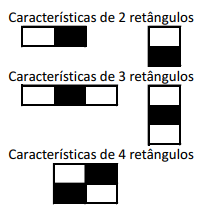
\includegraphics[width=0.3\textwidth]{Haarf.png}   
	\caption{Haar-like Features}
	\label{fig:figura2}
\end{figure}

Os retângulos pretos correspondem a um grupo de \textit{pixels} com tonalidade escura, ao passo que os retângulos brancos correspondem aos \textit{pixels} com tonalidade clara. Cada característica é definida por um valor que é obtido pela diferença entre o somatório das intensidades dos \textit{pixels} contidos na área preta e o somatório dos \textit{pixels} da área branca. Quando este valor é superior a um limiar padronizado, diz-se que a característica está presente na imagem. A figura \ref{fig:figura3} é um exemplo de aplicação desse conceito: há a utilização de uma característica de três retângulos (sendo dois pretos e um branco) para verificar se a imagem contem olhos, isso porque, normalmente, a região dos olhos é mais escura que a região superior do nariz. Em outras palavras, para que a existência de olhos seja detectada é necessário que uma característica com aquele formato específico possua um valor superior ao limiar determinado em treinamento.

\begin{figure}[!ht]
	\centering
	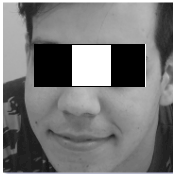
\includegraphics[width=0.3\textwidth]{exemplo_haar_features.png}   
	\caption{Exemplo de Haar-like Features}
	\label{fig:figura3}
\end{figure}

A Imagem Integral é uma técnica desenvolvida por \citep{Viola2001} para agilizar o cálculo das características. Para tanto, cria-se uma imagem intermediária tal que o valor de qualquer \textit{pixel} na posição (x,y) é dado pelo somatório dele com todos os \textit{pixels} localizados acima e a esquerda dele. Dessa forma, não é necessário acessar o valor de cada \textit{pixel} para calcular o valor de uma área. A figura \ref{fig:figura4} ilustra o funcionamento dessa técnica: nesse exemplo uma imagem está sendo representada por uma matriz 4x4, a qual contém uma região destacada cujo valor se deseja obter, note que o valor da soma dos \textit{pixels} dessa área já está definido na imagem integral, na última posição que define a área escolhida (sempre localizado no canto inferior direito).

\begin{figure}[!ht]
	\centering
	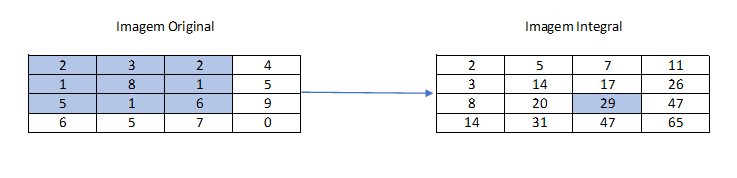
\includegraphics[width=1.0\textwidth]{imagem_integral.png}   
	\caption{Exemplo de Imagem Integral}
	\label{fig:figura4}
\end{figure}

Foi exposto anteriormente que a associação de características a objetos está condicionada a um treinamento. Essa tarefa é realizada pelo algoritmo de aprendizado de máquina supervisionado \textit{Adaboost}, cujo objetivo é construir um conjunto de classificadores simples, sendo cada um composto por apenas uma característica importante para a detecção do objeto, \citep{Viola2001}. Essa tarefa é importante porque em uma imagem existe uma grande quantidade de características (\textit{Haar-like features}) e, por isso, encontrar os tipos de características que melhor representam o objeto alvo economiza o esforço de analisar todas as demais. A \textit{Haar-like feature} da figura \ref{fig:figura3} é um exemplo de característica que compõe um classificador simples, pois ela sozinha não define uma face, mas a sua ausência já descarta a possibilidade de ser um rosto. Assim, o treinamento desse algoritmo consiste, segundo \citep{open2018}, na exposição de algumas centenas de amostras de um objeto específico, como um rosto ou um carro, chamados de exemplos positivos, os quais são formatados para terem as mesmas dimensões para só então compará-los com imagens arbitrárias de outros objetos de mesmas dimensões, chamados de exemplos negativos. Dos exemplos positivos, portanto, são definidos os classificadores (características e limiares).

Terminado o treinamento, é possível aplicar o classificador numa imagem de entrada. Quando o valor do conjunto de características que compõem o classificador é superior ao seu limiar, este atribui o valor 1 a imagem, o que indica que o objeto alvo está presente na imagem, caso contrário atribui 0, \citep{open2018}. Na detecção facial, esse processo ocorre diversas vezes por meio da combinação dos classificadores em cascata, que consiste no encadeamento de vários classificadores simples aplicados em sequência em uma imagem, que crescem em complexidade a cada iteração,  até que essa região seja rejeitada, por algum classificador, ou aprovada em todos os classificadores, \citep{open2018}. Quando a imagem é rejeitada por algum classificador simples, o processo encerra sem que os outros classificadores sejam aplicados. Esse procedimento aumenta drasticamente o desempenho e a precisão da detecção do objeto, pois as imagens indesejadas são eliminadas nas iterações iniciais, envolvendo menor processamento, sobrando para os classificadores mais complexos apenas aquelas com alta probabilidade de ser o objeto procurado.

Dessa forma, o papel a ser desenvolvido pelos algoritmos citados no início dessa seção é apoiar o reconhecimento facial, a partir da detecção de faces em imagens captadas por uma câmera fotográfica, as quais serão processadas e armazenadas para posterior análise dos algoritmos de reconhecimento facial que serão o objeto da seção seguinte.
\newpage
\section{Algoritmos de Reconhecimento Facial}
\noindent
Concluída a etapa de detecção facial, tem-se como produto a imagem da face já redimensionada, transformada para a escala de cinza e recortada da imagem original, esse processo é ilustrado na figura \ref{fig:figura25}, em (b) ocorre a transformação para a escala cinza (o retângulo vermelho é apenas uma abstração utilizada para representar a borda do que se irá recortar), e em (c) o recorte propriamente dito. A partir daí começa a etapa de reconhecimento que possui, basicamente, duas modalidades: autenticação e identificação. A primeira consiste em uma comparação 1 X 1 entre a imagem de entrada com a imagem da pessoa a ser autenticada. A segunda consiste em uma comparação 1 X N na qual a entrada é comparada com todas as imagens de um determinado conjunto para determinar se alguma pessoa do conjunto corresponde à entrada \citep{tdc2018}. No processo de apuração de faltas, convém utilizar apenas a modalidade de identificação.

\begin{figure}[!ht]
	\centering
	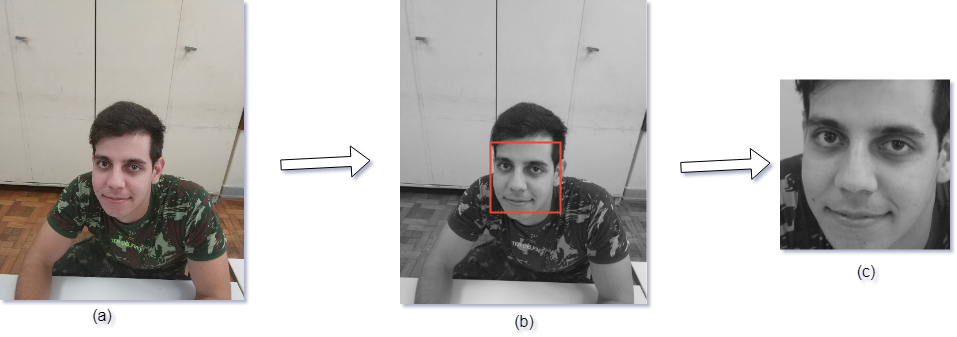
\includegraphics[width=1\textwidth]{processoRecorte.png}   
	\caption{Processo de recorte}
	\label{fig:figura25}
\end{figure}

Para o cumprimento da tarefa de reconhecimento facial, a biblioteca OpenCV  oferece três algoritmos: \textit{Eigenfaces}, \textit{Fischerfaces} e o LBPH. Por fazerem parte de uma biblioteca de código aberto, esses algoritmos são gratuitos para uso e esse fato contribuiu para a sua popularização, tendo como resultado o seu uso frequente em trabalhos científicos. Outro fator motivador para o emprego desses algoritmos é o seu bom desempenho, pois quando comparado ao MATLAB, que também pode ser utilizado para essa função, o OpenCV se destaca por usar menos memória e ser mais rápido que o seu concorrente, pois pode processar 30 quadros por segundo, enquanto o MATLAB executa de 3 a 4 quadros por segundo \citep{Kriti2018}. 

Quanto aos algoritmos, observou-se que em trabalhos científicos cujo objetivo é realizar o controle de faltas por meio de reconhecimento facial, o LBPH é apontado como a melhor opção dentre os três. Isso porque os algoritmos que utilizam as técnicas de PCA e LDA (Eigenfaces e Fisherfaces, respectivamente) para o reconhecimento facial apresentam dificuldades para superar problemas como a variação de: dimensionamento, iluminação, rotação e oclusão \citep{varun2018}. O trabalho de \citep{Kriti2018} também indica a superioridade do LBPH, o qual é classificado como o algoritmo mais eficiente e preciso, do OpenCV, para a tarefa de reconhecimento, após fazer um teste de desempenho comparando os três algoritmos. Esse teste também apontou a invariância à iluminação do LBPH, especialmente quando aplicado em imagens na escala de cinza, bem como a interferência mínima de ruídos. 

%Devido a essa robustez a variações, o LBPH foi o algoritmo escolhido para o desenvolvimento do presente projeto.


\subsection{Local Binary Patterns Histograms}
Descrito inicialmente em 1994, a operação LBP ficou conhecida como uma poderosa ferramenta de classificação de texturas, a qual teve a sua performance de detecção melhorada consideravelmente quando passou a ser combinada com histogramas de gradientes orientados \citep{tdc2018}. Com o uso dos histogramas o algoritmo é chamado de LBPH. O seu funcionamento possui 4 fases: treinamento do algoritmo, aplicação da operação LBP, extração de histogramas e reconhecimento de face.

O treinamento funciona de forma semelhante ao que foi descrito nos algoritmos de detecção, porém as imagens que compõem a base de dados são das pessoas a serem reconhecidas. Além disso, cada foto do arquivo precisa de uma identificação, podendo ser um número ou o nome da pessoa, que dever ser a mesma para todas as fotos. Isso é feito para que o algoritmo associe a uma mesma identificação as diversas expressões que uma pessoa possa fazer, aumentando, portanto, a probabilidade de reconhecimento.

A forma básica da operação LBP consiste em classificar os \textit{pixels} de uma imagem da seguinte maneira: a partir de uma região contendo 9 \textit{pixels}, que são representados por uma matriz 3 X 3, com cada \textit{pixel} assumindo um valor, correspondente a intensidade de cor, entre 0 e 255 (correspondentes aos tons de cinza). Em seguida usa-se o valor central da matriz como limiar para definir um novo valor, agora binário, para os outros 8 vizinhos. Caso o valor do \textit{pixel} vizinho seja menor que o valor do limiar, atribui-se o valor 0, caso contrário o valor é 1. O próximo passo é concatenar os valores para ter uma sequência binária (daí o nome padrão binário local), que é convertida para um número decimal que passa a representar o conjunto de \textit{pixels}, \citep{tdc2018}. A figura \ref{fig:figura6} ilustra esse processo. A forma mais genérica da operação LBP usa vizinhanças circulares, figura \ref{fig:figura7} , as quais podem abranger qualquer quantidade de vizinhos com a variação do raio, definidos pelo usuário, por meio de uma interpolação bilinear dos valores dos \textit{pixels} \citep{Timo2006}.

%Com relação ao funcionamento do algoritmo, inicia-se a partir de uma imagem na escala de cinza,
\begin{figure}[!ht]
	\centering
	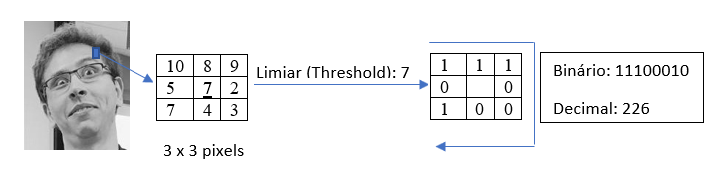
\includegraphics[width=1.0\textwidth]{lbpV1.png}   
	\caption{Operação LBP}
	\label{fig:figura6}
\end{figure}

\begin{figure}[!ht]
	\centering
	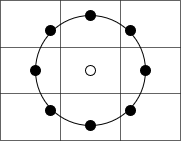
\includegraphics[width=0.25\textwidth]{vizicircular.png}   
	\caption{Operação LBP - vizinhança circular}
	\label{fig:figura7}
\end{figure}

O procedimento seguinte é a extração dos histogramas, que consiste em agrupar os valores dos \textit{pixels }classificados pela operação LBP, de forma que para cada região da imagem haverá um histograma contendo a quantidade de ocorrências de cada tom de cinza presente. Essas regiões que dividem a imagem são chamadas de \textit{grids}, pois têm o mesmo aspecto de uma grade, e podem ter qualquer formatação quanto a quantidade de linhas e colunas: nas linguagens de programação os parâmetros que definem a quantidade de \textit{grids} são \textit{Grid x} e \textit{Grid y}. Os histogramas extraídos de cada \textit{grid} representam características locais, contendo 256 posições (de 0 a 255) relativas aos diversos tons de cinza. Em seguida, todos os histogramas locais são concatenados, gerando um histograma global que representa as características da imagem principal, conforme pode ser vista na figura \ref{fig:figura8} , \citep{Timo2006}. Dessa forma, para uma imagem de 9 x 9 \textit{grids}, tem-se um histograma de 20.736 posições (9x9x256). \newpage

\begin{figure}[!ht]
	\centering
	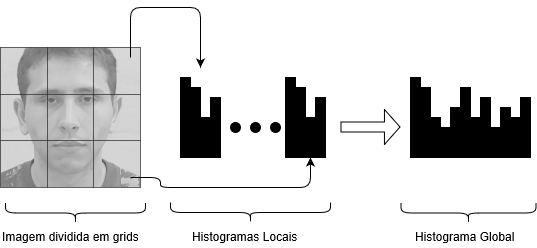
\includegraphics[width=0.7\textwidth]{lbphC.png}   
	\caption{Extração de Histogramas}
	\label{fig:figura8}
\end{figure}

O reconhecimento facial se dá, portanto, pela comparação entre os histogramas globais: da imagem de entrada com as imagens do conjunto de treino. O parâmetro de comparação utilizado é a distância entre os vetores de características, que são as estruturas de dados usadas para armazenar a informação dos histogramas. Na implementação do LBPH do OpenCV existem 4 métodos para o cálculo dessa distância: a distribuição qui-quadrado, a distância euclidiana, a distância euclidiana normalizada ou a fórmula do valor absoluto \citep{open2018}. Após o cálculo das distâncias entre a imagem de entrada e as imagens do banco de dados, o algoritmo retorna a identificação da imagem que apresenta a menor distância em relação à imagem de entrada. %$D = \sqrt[]{\sum_{i=1}^{n}(hist1_{i} - hist2_{i})^{2}}$

